\documentclass[10pt,a4paper]{article}

%% PACKAGES WITH OPTIONS
\usepackage[english]{babel}
\usepackage[T1]{fontenc}
\usepackage[utf8]{inputenc}
\usepackage[version=4]{mhchem} % Chemistry and isotopes with \ce{} (other option: 'chemformula' \ch{})
\usepackage[numbers]{natbib} % numbers: needed argument, otherwise error
\usepackage[section]{placeins} % Place floats in their own section
\usepackage[nottoc,notlot,notlof]{tocbibind} % Include bibliography in table of contents

%% PACKAGES WITHOUT OPTIONS
\usepackage{adjustbox} % Use \begin{adjustbox}{center} environment for too wide floats
\usepackage{amsmath, amsfonts, amssymb}
\usepackage{ctable} % Usage: \ctable[options]{coldefs like c|c|r|l}{\tnote commands for footnotes}{normal table content}, with \tnote[symbol]{text} footnote definitions, and \tmark[symbol] used to reference the footnote in the normal table content
\usepackage{enumitem} % Lists
\usepackage{flafter} % Place floats after their first appearance in text
\usepackage{float} % [H] modifier for floats etc.
\usepackage{graphicx}
\usepackage{hyperref, cleveref} % Creates links (boxes in various colors around words)
\usepackage{indentfirst} % Always indent the first line of a section
\usepackage{listings} % Typesetting source code
\usepackage{physics} % Vector calculus etc.
\usepackage{siunitx} % Fancy display of SI units
\usepackage{subcaption} % Enables subfigures
\usepackage{titling}
\usepackage{xcolor} % Anything with color e.g. \fcolorbox{black}{red}{}
\usepackage{xurl} % Loads package 'url' and breaks urls nicely

%% PACKAGES SETUP COMMANDS
\hypersetup{colorlinks=true,urlcolor=blue,citecolor=gray}

%% COMMANDS
% Bold and italic vector symbols (preferably use \vb{} instead)
\renewcommand{\vec}[1]{\boldsymbol{#1}}
% Monospaced inline code (for multiline code, use package 'listings')
\newcommand{\code}[1]{\texttt{#1}}
% Equals sign, with number above referencing some equation
\newcommand{\numeq}[1]{\stackrel{\scriptscriptstyle(\mkern-1.5mu#1\mkern-1.5mu)}{=}}
% If-and-only-if sign, with number above referencing some equation
\newcommand{\numiff}[1]{\stackrel{\scriptscriptstyle(\mkern-1.5mu#1\mkern-1.5mu)}{\Leftrightarrow}}
% Numbers a single line in a no-numbering multiline equation* or align*
\newcommand{\numberthis}{\addtocounter{equation}{1}\tag{\theequation}}
% MuMax3
\newcommand{\mumax}{$\mathsf{mumax}^3$}

%% TITLE VARIABLES
\author{Jonathan Maes}
\title{Biaxial nanomagnets as building block for balanced half-adders}


\begin{document}

\begin{titlingpage}
\maketitle
\end{titlingpage}

\newpage
\pagenumbering{roman}

\tableofcontents
\newpage
\pagenumbering{arabic}

This thesis makes use of the \mumax{} micromagnetic simulation tool~\cite{MuMax3}.
Gilbert is \cite{Gilbert1956} and Lifdau is \cite{LANDAU1992}.

Interesting sources regarding the random thermal switching could be \cite{ThermFluc_SingleDomain, RandomSwitch_MonteCarlo, Nonmonotonic_reversal}, and perhaps \cite{MagDynamics_JumpNoise}.
Exchange bias is explained in \cite{ExchangeBias, ExchangeBias_nanostructures, ExchangeBias_Mechanisms}.
Quantum Cellular Automata (QCA) are discussed in \cite{QCA_Algorithms, QCA_GameOfLife}. Magnetic QCA (MQCA) are discussed in \cite{MQCA_MajorityGate, MQCA_RoomTemp, MQCA_ImageRecognition}.

\section{Introduction}
%\noindent \textit{Note: This section exists to explain nanomagnetic logic to the unfamiliar reader. \textbf{Biaxial island} begins the investigation of the dynamics of a single biaxial island, and is a suitable starting point for those already familiar with nanomagnetic logic.} \bigskip

\noindent An atom may display what is called a \textbf{magnetic dipole moment}, on one hand due to the angular momentum of electrons around the nucleus, and on the other hand due to the intrinsic spin of the elementary particles which make up the atom. The magnetic moment can be defined using the torque the atom experiences in a magnetic field.~\cite{IntroMagneticMaterials} In a material, many atoms are together, and the macroscopic sum of all their magnetic moments is called the magnetization of the material. In a crystalline material, the periodicity of the lattice can give rise to specific orderings of the magnetic moments, like for example ferromagnetism where all individual magnetic moments of neighboring atoms try to align themselves in the same direction. \par 
Such a ferromagnetic material, like iron, nickel or cobalt, consists of many \textbf{magnetic domains}. Each domain, on the order of several tens of micrometers, has a nearly uniform magnetization pointing in a random direction. Because the direction of each domain is random, a ferromagnetic material does not display a macroscopic net magnetization. However, when one fabricates a very small island of several hundred nanometers made of such a ferromagnetic material, it will not be made up of several domains, but rather only one, and will thus have a nearly uniform magnetization. \par
If this island has one or another form of anisotropy, be it due to the crystal structure or the shape of the island, the magnetization will have minimal energy if it lies along a certain axis, called the `easy axis'. \textbf{Shape anisotropy} originates from the observation that the magnetization of a domain preferably orients itself along the long axis of a microscopic structure. An example that is often used is a 2D ellipse, as this can easily be produced via electron beam lithography, for which the easy axis is equal to the long axis of the ellipse. In general, if a structure has one easy axis (and thus two stable directions), we speak of uniaxial anisotropy. In the case of two easy axes (and thus four stable directions), as will be the main topic of this thesis, this is called biaxial anisotropy. Biaxial shape anisotropy can be achieved with a geometry that is invariant under rotation of \SI{90}{\degree}. \par
In the uniaxial case, there are two stable directions, which can be related to a `0' or `1' bit. Hence, these nanomagnetic islands can be used to create a \textbf{digital logic circuit}. There have been examples in literature where majority logic gates and NAND gates have been created using nanomagnets.~\cite{GYP-18} Biaxial nanomagnets can be used to encode two bits in one island, because those have 4 stable magnetization directions. This should allow for smaller logic gates due to the increased integration density as compared to uniaxial islands. The goal of this thesis is to create a half adder using biaxial nanomagnets. Because a half adder takes two bits as input and yields two bits as output, it almost feels natural to design it using biaxial nanomagnets instead of uniaxial ones.
% TODO: talk about making logic devices with this
In the following sections, the nature of magnetism and magnetic domains, quantum cellular automata, signal propagation and techniques for imaging the magnetization will be explained in more detail.

\subsection{Domains}
In 1907, Weiss proposed the idea that a ferromagnetic material contains several uniformly magnetized domains, but that the magnetization of each domain individually is random, thus resulting in a macroscopic zero net magnetization of a large amount of material.~\cite{MuMax3_advances} These domains should not be confused with grains, which are only related to the crystallography. The uniform alignment inside a single domain is due to the quantum mechanical Heisenberg-Dirac exchange interaction.~\cite{MuMax3_advances, heisenberg1928theorie} The magnetostatic energy makes it unfavorable for neighboring moments to align themselves parallel to one another, which competes with the exchange energy which tends to align neighboring moments in the same direction. Since the exchange energy only works on small length scales, domains are formed under the influence of the exchange energy, while different domains tend to cancel out their fields due to the magnetostatic energy. The typical size of these domains is on the order of several tens of micrometers. When the size of the material becomes on the order of micrometers, the domains form very symmetric patterns in order to minimize their energy, and on even smaller length scales only one domain remains.~\cite{NML_Carlton} So, if one makes a droplet of ferromagnetic material smaller than this typical size, the droplet will have a nearly uniform magnetization, with a magnitude equal to the saturation magnetization of the material.~\cite{NML_Carlton} Such a small droplet can for example be defined using electron beam lithography.~\cite{MQCA_RoomTemp, NML_Carlton} By introducing anisotropy in the droplet, which can be either magnetocrystalline or shape anisotropy, one or more axes can be made energetically favorable for the magnetization to align itself along. Magnetocrystalline anisotropy favors the crystal axes. Shape anisotropy can be realized by giving the droplet an elliptical shape instead of a perfect circle. In the uniaxial case, there is one stable magnetization axis, and the two directions `up' and `down' along this axis can be related to bits `0' and `1'.~\cite{MQCA_RoomTemp} This is not to be confused with unidirectional anisotropy, which only has one stable magnetization direction, and can be achieved using the exchange bias effect.~\cite{ExchangeBias_Mechanisms,ExchangeBias_nanostructures,ExchangeBias} A lot of research has been conducted to use uniaxial anisotropy for computation, and logic gates and wires have been proposed, which use classical magnetostatic interactions to propagate the information.~\cite{GYP-18,MQCA_MajorityGate,SwitchingForced_EnergyEfficient} The use of two favorable axes, i.e. biaxial anisotropy, allows for a higher logic density, as the four stable directions `up', `down', `right' and `left' can be related to `00', `01', `10' and `11'.~\cite{MQCA_ImageRecognition} This can occur for cubic crystals, and can also be realized by giving the shape of the droplet more symmetry, for example by making the shape the union of two ellipses.


\subsection{Quantum Cellular Automata}
Traditional digital logic technologies like CMOS use field-effect transistors to control the flow of electrons. This kind of architecture fundamentally only allows information to flow in one direction. Other architectures allowing communication between the output and input in both ways could allow certain types of computations to be executed faster. One approach to realizing such an architecture are the Quantum Cellular Automata (QCA), which use quantum effects, in a broad sense, to make logic gates. A cellular automaton is a mathematical concept, proposed by Von Neumann~\cite{Sideinfo_SelfRepAutomata}, in which the universe is divided into a regular grid of cells, where each cell is influenced by its direct neighbors. The most famous example of such a mathematical cellular automaton is Conway's Game of life, which has been shown to be universal for computation, as any Turing machine can be encoded in it.~\cite{QCA_GameOfLife} Apart from the universality in the Turing sense, cellular automata provide an additional benefit because they are able to process algorithms in a distributed manner due to the spatial parallelism inherent to them.~\cite{QCA_GameOfLife} From a practical point of view, QCA can be orders of magnitude smaller and more energy efficient than traditional CMOS technology.~\cite{MQCA_RoomTemp} \par
There are several possibilities to realize QCA, which can generally be classified as either electronic or magnetic QCA. Electronic QCA (EQCA) make use of the forces between electrons, while magnetic QCA (MQCA) leverage the magnetic moments of atoms. EQCA are called ``quantum'' because they use quantum mechanical tunneling of charge between quantum dots, MQCA are quantum because of the exchange interaction between individual atomic magnetic moments.~\cite{MQCA_RoomTemp} Apart from this quantum nature of the building blocks, QCA are essentially classical devices switching through either coulombic or magnetic interactions.~\cite{QCA_Algorithms} What all these QCA have in common, is that every fundamental building block (electrons, magnetic moments...) of these automata influences every other building block in the automaton, thus allowing the aforementioned two-way flow of information between what would traditionally be referred to as input and output. The MQCA are the main subject of this paper, but it is interesting to take a short look at EQCA as well, for both share some ideas and problems. \par
% Small segue to quantum dot cellular automata
One specific implementation of EQCA makes use of square cells, each with four quantum dots at the vertices of a square. These quantum dots can accomodate an electron, and each cell is made such that there are always two excess electrons present. It is then energetically favorable for these electrons to occupy two diagonal quantum dots.~\cite{QCA_DigitalLogicGate} The two diagonal configurations are then the `0' and `1' states. An extensively studied logic gate using this architecture is the three-input majority logic gate. It consists of five cells arranged in a plus-shape, with three inputs and one output. Just like the familiar NAND gate, the majority gate is universal for computation.~\cite{NML_Carlton} By fixing one of the inputs to 0 or 1, an AND or an OR operation can be realized, respectively. A drawback for these EQCA is that they require low electron temperatures in order to work reliably, as otherwise thermal smearing of the charge states of the dots becomes an issue.~\cite{QCA_DigitalLogicGate} \par
QCA compute by relaxing to a configuration of minimal energy.~\cite{QCA_Algorithms} It is important that all these relaxed configurations are equal in energy level. This is what is meant by `balanced' QCA. A necessary condition for an automaton to be balanced is that the number of distinguished configurations with minimum energy should be equal to the number of input combinations the automaton handles.~\cite{QCA_Algorithms}


\subsection{Nanomagnetic islands}
As was mentioned before, the magnetization of a nanomagnetic island likes to align itself along the longest axis of the shape. This can be understood as follows. Consider a theoretically ideal island so small that it only consists of two atoms, and thus only two magnetic moments. Three different situations are then shown in~\cref{fig:Intro_IslandEllipticPreferredDirection}.
The first configuration has both moments vertical and in the same direction, which makes their magnetic fields nicely lined up, hence this is a low energy state. The second configuration has the magnetic moments in opposite directions, such that their fields oppose each other, which is not a low energy configuration. The third configuration has both moments horizontal and oppositely directed, which once again has the magnetic fields nicely lined up in a low energy state. In the fourth configuration they are pointed horizontal and in the same direction, so the fields once again oppose each other and we do not have a low energy state. Thus, only two of these four configurations are energetically favorable. Now note that we are only dealing with ferromagnetic materials, which have the property that neighboring moments like to align themselves in the same direction, due to the exchange energy (\cref{par:Energy_Exchange}). This only leaves the first situation as a stable one, hence explaining the \textbf{tendency for ferromagnetic materials to be magnetized along the long axis of a microscopic geometric structure}. In larger geometric structures however, the third configuration is a perfectly acceptable way for two separate domains to align themselves, but in this thesis we are only dealing with small single-domain islands. \par
\begin{figure}[t]
    \centering
    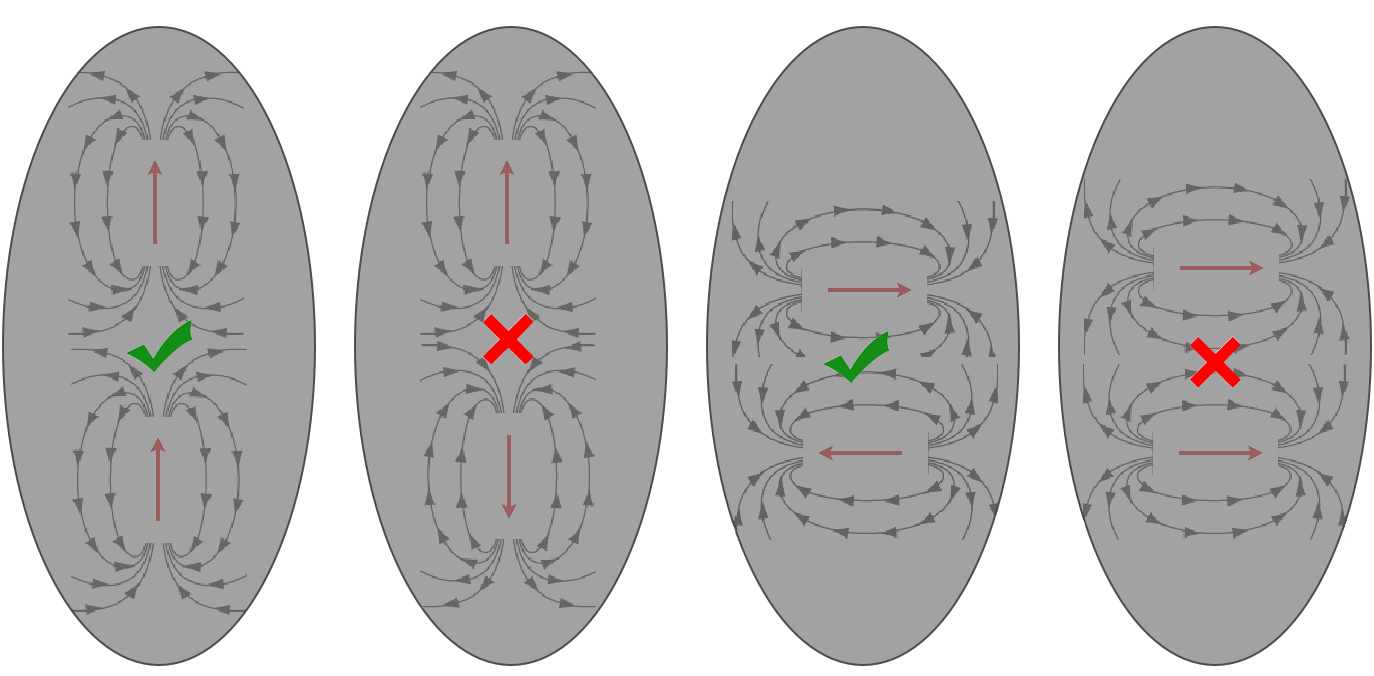
\includegraphics[width=0.9\columnwidth]{Figures/Introduction/NML_Carlton - Figure 1.9 adapted.png}
    \caption{Theoretical situation where an island is made up of two magnetic moments, for four different configurations, explaining the tendency for ferromagnetic materials to be magnetized along the long axis of a microscopic geometric structure. Figure adapted from fig. 1.9 in \cite{NML_Carlton}.}
    \label{fig:Intro_IslandEllipticPreferredDirection}
\end{figure}
In case of higher symmetry, for example with biaxial shape anisotropy, it is no longer clear which symmetry axes will be the easy axes, and which the hard ones, as will be examined in more detail in \cref{par:Biaxial_island}.

\subsection{Signal Propagation}
Nanomagnetic logic gates need to be able to communicate with each other in order to form a larger and more useful circuit. For this, nanomagnets are placed next to each other, such that they form a sort of chain. Signal propagation through chains of nanomagnets does however come with some large complications. One of the advantages of nanomagnetic logic is that different islands influence each other, but this bidirectional interaction causes problems when trying to propagate signals. Let us start with examining the uniaxial case, as this has been studied most intensively, and then extend our knowledge to biaxial signal propagation.
\subsubsection{Uniaxial}
In the uniaxial case, a wire can be formed by placing elliptic islands next to each other, either along their hard axes (\cref{fig:Intro_IslandEllipticChainGeometries}, left) or along their easy axes (\cref{fig:Intro_IslandEllipticChainGeometries}, right). In the first case, neighboring islands will try to align in opposite directions, in the second case they want to align in the same direction. Let us consider the first case now, as the second case is very similar. % TODO: is the other case extremely similar? I guess so, but I want to see evidence of this because in NML they use additional stabilizers for that configuration, so best to talk about that later.
\begin{figure}
    \centering
    
\includegraphics[width=0.5\columnwidth]{Figures/Introduction/Chains_geometries.pdf}
    \caption{Two possible chain geometries for uniaxial islands. Left: chain along the islands' hard axis. Right: chain along the islands' easy axis.}
    \label{fig:Intro_IslandEllipticChainGeometries}
\end{figure}
Suppose the wire has been initialized with a `1'. Then all following moments will be in alternating directions, as shown in the top of \cref{fig:Intro_SolitonRandomWalk}. Now the input bit is changed to a `0' and we wish to propagate this signal through the wire, as shown in the middle of \cref{fig:Intro_SolitonRandomWalk}. The second magnetic moment now wants to align itself up due to its left neighbor (the input bit), but also wants to align itself down due to its right neighbor. As such, no net force acts on the second bit and it will randomly switch. Such a `defect' in the wire is called a magnetic soliton.~\cite{MQCA_RoomTemp} As soon as this second bit changes, the third bit is now in a similar situation, as shown at the bottom of \cref{fig:Intro_SolitonRandomWalk}, and the soliton has moved one place to the right. Now both the second and third bit have an equal chance of switching, and thus the signal has an equal chance of propagating forward to the output (third bit switches) or backward to the input (second bit switches). Thus, the signal (or, equivalently, the soliton) will perform a random walk along the wire. If the input bit is forced to remain `0', the signal will thus reach the output after a time proportional to the square of the number of nanomagnets the chain consists of.~\cite{Wolfram_RandomWalk} It is clear that this is not ideal, and several techniques have been proposed to force the signal to propagate along the wire in one direction. 
\begin{figure}
    \centering
    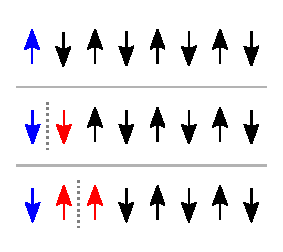
\includegraphics[width=0.5\columnwidth]{Figures/Introduction/Soliton_random_walk_2steps.pdf}
    \caption{Blue arrows are the input bits. Red arrows have no preferred direction due to competing interactions of their neighbors. A dotted line indicates the location of a magnetic soliton. Top: initial ordering of the wire for a `1' (up) input. Middle: input bit changes to `0' (down), causing no net force to act on the second island. Bottom: second island randomly switches, causing no net force to act on the third island anymore either.}
    \label{fig:Intro_SolitonRandomWalk}
\end{figure}

One technique makes use of an external magnetic field to initialize each island along its hard axis whenever a new bit needs to be propagated. This can be seen as a form of clocking. The first island is initialized in either the `0' or `1' state and functions as an input bit. Keeping this first bit intact under an external field can for example be achieved with the exchange bias effect.~\cite{ExchangeBias_Mechanisms,ExchangeBias_Mechanisms,ExchangeBias} When the external field is removed, each subsequent island chooses a direction to fall onto its easy axis. If this happens adiabatically, each island will fall in the correct direction and no solitons appear.~\cite{NML_Carlton} \par
However, thermal fluctuations can cause some islands to fall in the wrong direction, which can be problematic. It can therefore be instructive to release the islands one at a time to ensure the correct behavior by propagating the signal along the wire one nanomagnet at a time. Furthermore, the use of an external magnetic field to control the wire is not very `clean', because a large external field will affect all the wires in the circuit. One possible solution is to manufacture the nanomagnetic island with a piezoelectric layer underneath, which can induce strain in the island, which exerts a force on the magnetization as will be explained in \cref{par:Energy_MagnetoElastic}. Each nanomagnet can then be controlled electronically. Another possibility is to place the nanomagnetic island between two special electrodes which produce a spin-polarized current. These electrons can then exert a torque on the magnetization, known as the spin transfer torque.~\cite{SwitchingForced_EnergyEfficient,syllabus_PoAEaPD}

\subsubsection{Biaxial}
% TODO: Section on biaxial situation (seems like biaxial is less easy to find information about than uniaxial so need to find some more papers for that)

\subsection{Imaging the magnetization}
If one wishes to not only perform theoretical, but also practical studies on nanomagnetic islands, specialized microscopy techniques can be useful for imaging the magnetization direction. Three often encountered techniques are presented in this section, each with certain advantages and disadvantages.
\subsubsection{Magnetic Force Microscopy}
Magnetic Force Microscopy (MFM) is a form of scanning probe microscopy that can measure out-of-plane magnetic fields. For this, a cantilever with a magnetic tip is used which is scanned across the sample at a very low height. One must take care that this magnetic tip does not significantly influence the magnetization of the sample itself.~\cite{Probing_MagnetoOptics} Also, if this tip were to simply scan over the surface, both the magnetic forces as well as the atomic forces would be measured. As we want to determine only the magnetic field, the topography of the sample is first determined using conventional Atomic Force Microscopy.~\cite{PEEM, NML_Carlton} Once the topography is known, the magnetic tip can scan the sample while maintaining a constant distance above it using the known topography. This decouples the measurement of magnetic forces from the atomic forces and allows one to determine just the magnetic field. Important to note is that the force measured is only the out-of-plane component of the magnetic field, because the cantilever can only move vertically and is thus only sensitive to the vertical component of the magnetic field.~\cite{NML_Carlton} \par
Because there are strong out-of-plane components on either end of a nanomagnet, when imaged using MFM one such island will manifest itself in the output as the combination of a region with positive and a region with negative out-of-plane magnetic field, because the stray magnetic field of a dipole curls back on itself.~\cite{NML_Carlton} \par % TODO: show nice example of MFM image
A disadvantage of MFM is that it does not image the magnetization directly, but rather the stray out-of-plane magnetic fields, which can make the results more difficult to interpret. It is however a cheaper technique that requires less safety measures than X-ray based techniques, which are discussed in the next section.

\subsubsection{Photoemission Electron Microscopy using X-ray Magnetic Circular Dichroism}
Photoemission Electron Microscopy (PEEM) is a microscopy technique which images secondary electrons emitted from the sample upon irradiated with X-rays. This kind of electron microscopy can achieve a high spatial resolution of less than \SI{50}{\nano\metre}, with a typical probing depth in metals of about \SI{2}{\nano\metre}.~\cite{PEEM} The technique can be used to simply image the chemical and elemental structure of the sample, but can be adapted to image the magnetization direction in ferromagnets by utilizing an effect called X-ray Magnetic Circular Dichroism (XMCD). This is a physical phenomenon where the number of electrons emitted from the sample upon irradiation with circularly polarized X-rays depends on the magnetization direction of the surface of the sample.~\cite{NML_Carlton} More specifically, the quantity that is measured is the angle $\phi$ between the magnetization direction $\vb{m(\vb{r})}$ of the sample and the photon spin $\vec{\sigma}$, which is aligned with the photon propagation direction and changes sign when the photon helicity is reversed.~\cite{PEEM} The intensity of emitted electrons is given by
\begin{equation}
    I_{\mathrm{XMCD}} \propto M_S \cos(\phi) \mathrm{.}
    \label{eq:XMCD}
\end{equation}
This way, PEEM can directly measure the in-plane magnetization direction, which makes it easier to interpret than an MFM image. A slightly more detailed description of the geometry and image acquisition of this kind of electron microscope can be found in~\cite{PEEM}. % TODO: QUESTION: Is this an expensive method? I suppose MFM is relatively cheap, but this requires a synchrotron which many papers do at the so-called 'Swiss Light Source', which I suppose is one of the few places where they have this equipment?
% TODO: Show nice example of PEEM image

\subsubsection{Magneto-Optical Kerr Effect}
The Magneto-Optical Kerr Effect (MOKE) can also be used to determine the magnetization, albeit the average over a larger area on the order of several tens of \SI{}{\micro\metre\squared}. A linearly polarized laser beam is focused onto the sample, and the polarization state of the reflected light is measured in order to access the longitudinal Kerr effect.~\cite{MQCA_RoomTemp} The longitudinal Kerr effect says that, depending on the angle between the magnetization and the incoming light, the reflected light will become elliptically polarized to a certain degree.~\cite{KerrFaraday_book} This effect is small, but the ellipticity is directly proportional to the cosine of the angle, which can be used to derive the magnetization direction. There also exists the transversal Kerr effect, but this is not often used as it results in a change in reflectivity, which is more difficult to detect. \par 
The low resolution of this technique is due to the diffraction limit of the laser used, and for structures smaller than this diffraction limit the signal strength diminishes.~\cite{Probing_MagnetoOptics} One must take care that the focused laser beam does not excessively heat up the sample, as this could cause the measurement to influence the magnetization of the sample. The temperature rise for a \SI{2.5}{\milli\watt} laser was however found to be negligible.~\cite{Probing_MagnetoOptics} This measurement technique can be easier or cheaper to set up than the X-ray technique, but the (very) low resolution does not allow the imaging of individual nanomagnets in complex structures.

% TODO: To define the features: Electron beam lithography~\cite{NML_Carlton}, but i dont think there is a lot to say about that


\section{Physics}
% === THE FOLLOWING IS A NONCOMPREHENSIVE SUMMARY OF THE PHYSICS ===
The main formulae are derived in \cite{abert2013discrete} or \cite{NML_Carlton} and in the \mumax{} advances \cite{MuMax3_advances}. \par
In a crystalline material, the atoms are evenly spaced. Each atom has a discrete magnetic moment $\vb{m_i}$ associated with it. The interaction of many magnetic moments can give rise to macroscopic effects. Since every magnetic moment interacts with every other magnetic moment, the underlying problem is therefore a discrete N-body problem. Unfortunately, such a problem quickly becomes very hard if not impossible to solve analytically for even small $N$, hence restricting analytical calculations to very small systems.~\cite{abert2013discrete} Due to the lack of an analytical solution, many particular problems can only be solved approximately in a numerical manner.~\cite{abert2013discrete} Even with numerical techniques, the computational power or time required to solve an N-body problem increases rapidly with $N$, due to the number of interactions. For this reason, a continuum theory was developed, called the micromagnetic theory. In this formalism, the magnetization is represented by the continuous magnetization field, denoted by $\vb{M}(\vb{r}) = M_S \vb{m}(\vb{r})$. This is the magnetic moment per unit volume averaged over a small region of space, with $\vb{m}(\vb{r})$ a unit vector, and $M_S$ called the saturation magnetization.~\cite{Gilbert1956}
The size of this small region is characterized by the exchange length $\lambda$, a formula for which is given by \cref{eq:Energy_ExchangeEnergy_ExchangeLength}. It should be much smaller than the size of a single magnetic domain, yet much larger than a crystal unit cell, so on the order of several nanometres. It is clear that this continuum approximation is only applicable if locally all discrete magnetic moments try to align themselves parallel to each other, i.e.
\begin{equation}
    \vb{m_i} \approx \vb{m_j}~~\mathrm{if}~~\abs{\vb{r_i} - \vb{r_j}} < \lambda \mathrm{,}
\end{equation}
as is for example the case in ferromagnets.~\cite{abert2013discrete} \par
In situations where this approximation holds, the continuum theory can provide a significant computational improvement, because one can now use numerical cells with typical dimensions on the order of $\lambda$, which significantly decreases the amount of variables compared to the original N-body problem, where every single atom had to be taken into account. The characteristic size of a simulation using micromagnetic theory is on the order of tens to hundreds of nanometres, using millions of cells with dimensions on the order of $\lambda$.~\cite{abert2013discrete} Thus, the micromagnetic theory works well on a macroscopic scale and can be solved numerically in a reasonable amount of time, which would be wholly impossible with an N-body approach.


\subsection{Energy contributions}
The energy corresponding to a certain continuous magnetization field $\vb{m}(\vb{r})$ is the sum of several different contributions
\begin{equation}
    E = E_{exch} + E_{anis} + E_{demag} + E_{Zeeman} + E_{me} \mathrm{.} \label{eq:Energy_Terms}
\end{equation}
The physical nature of these different terms along with small derivations to accomodate them to the continuum approximation are presented in this section.
\subsubsection{Exchange energy}
\label{par:Energy_Exchange}
The exchange energy is of quantum mechanical origin. It tries to align neighboring spins and takes on the simple form
\begin{equation}
    E_{i,j} = -J \vb{S_i} \vdot \vb{S_j} \mathrm{.}
    \label{eq:Energy_ExchangeEnergy_Discrete}
\end{equation}
Summing over all contributions gives
\begin{equation}
    E = -\sum_{i,j} J_{i,j} S^2 \vb{n_i} \vdot \vb{n_j} \mathrm{,}
    \label{eq:Energy_ExchangeEnergy_SumDiscrete}
\end{equation}
with $\vb{S_i} = S \vb{n_i}$ and $\abs{n_i} = 1$. 
The sign of $J$ determines whether the spins align parallel ($J>0$) or anti-parallel ($J<0$). A parallel alignment results in a so-called ferromagnetic material, while an anti-parallel alignment is characteristic of an anti-ferromagnetic material.
% TODO: Exchange bias? Hier misschien niet op zijn plaats maar heeft wel te maken met FM/AFM

Micromagnetic theory makes use of the magnetization field $\vb{m}(\vb{r})$, while \cref{eq:Energy_ExchangeEnergy_Discrete} is discrete. Two particles $i$ and $j$ only feel the exchange interaction when they are close to each other. This allows us to expand $\vb{m}(\vb{r}) \cdot \vb{m}(\vb{r} + \Delta\vb{r})$ in first order~\cite{abert2013discrete} to
\begin{align*}
    \vb{m}(\vb{r}) \cdot \vb{m}(\vb{r} + \Delta\vb{r}) &= 1 - \frac{1}{2}(\vb{m}(\vb{r}) - \vb{m}(\vb{r} + \Delta\vb{r}))^2 \\
    &\approx 1 - \frac{1}{2}\sum_i(\Delta\vb{r} \cdot \gradient{m_i})^2 \numberthis \label{eq:Energy_ExchangeEnergy_DotApprox} \mathrm{.}
\end{align*}
We can now write an equation similar to \cref{eq:Energy_ExchangeEnergy_SumDiscrete}, but for $\vb{m}(\vb{r})$:
\begin{equation*}
    E_{exch} = \int_\Omega \sum_i A_i \vb{m}(\vb{r}) \cdot \vb{m}(\vb{r} + \Delta\vb{r}_i) \mathrm{,}
\end{equation*}
which by substitution of \cref{eq:Energy_ExchangeEnergy_DotApprox} finally yields~\cite{abert2013discrete,Gilbert1956}
\begin{equation}
    E_{exch} = A_{ex} \int_\Omega \sum_i (\gradient{m_i}(\vb{r}))^2 \, d\vb{r} \mathrm{.} \label{eq:Energy_Term_Exchange}
\end{equation}
$A_{ex}$ is called the exchange stiffness constant.~\cite{Gilbert1956} The physical interpretation of this energy term is that the magnetization tries to align itself as smoothly as possible.
The exhange length $\lambda$ can now be calculated as
\begin{equation}
    \lambda = \sqrt{\frac{2 A_{ex}}{\mu_0 M_S^2}} \mathrm{.}
    \label{eq:Energy_ExchangeEnergy_ExchangeLength}
\end{equation} % TODO: find a reference which mentions this

\subsubsection{Anisotropy energy}
A material may exhibit anisotropy due to its crystal structure. The most often encountered types of anisotropy are uniaxial and cubic anisotropy. Uniaxial anisotropy is common in hexagonal or tetragonal crystal structures, while cubic anisotropy is often present in FCC or BCC structures.~\cite{Gilbert1956, abert2013discrete} \par
In the uniaxial case, the energy is minimal when the magnetization lies along a certain axis $\vb{u}$. In the cubic case, there are three such axes $\vb{e_i}, i=1,\dots,3$, which are all equivalent. The direction of $\vb{M}$ along this axis (i.e. $\vb{m}=\pm \vb{u}$) does not matter, such that $E(\vb{m}_{min}) = E(-\vb{m}_{min})$. For this reason, only even orders in the Taylor expansion are considered.~\cite{abert2013discrete} For uniaxial anisotropy this gives
\begin{equation}
    E_{anis,u} = - \int_\Omega \big(K_{u1} (\vb{m} \cdot \vb{u})^2 + K_{u2} (\vb{m} \cdot \vb{u})^4 + \dots\big) \, d\vb{r} \mathrm{.} \label{eq:Energy_Term_AnisUniaxial}
\end{equation}
For cubic anisotropy, one can use a similar symmetry reasoning~\cite{abert2013discrete} to find
\begin{equation}
    E_{anis,c} = \int_\Omega \big(K_{c1} (m_1^2m_2^2 + m_2^2m_3^2 + m_3^2m_1^2) + K_{c2} m_1^2m_2^2m_3^2\big) \, d\vb{r} \mathrm{,} \label{eq:Energy_Term_AnisCubic}
\end{equation}
with $m_i(\vb{r}) = \vb{m}(\vb{r}) \cdot \vb{e_i}, i=1,\dots,3$.

\subsubsection{Demagnetization energy/Magnetostatic energy}
The demagnetization energy, often also called the magnetostatic energy, is the energy arising from the interaction of every magnetic moment in a ferromagnetic material with the force of every other magnetic moment in the material.~\cite{NML_Carlton} In other words, it is the energy of the magnetization in the magnetic field created by itself.~\cite{abert2013discrete}
From classical electrodynamics it is known that, in the absence of currents,
\begin{align}
	\div{\vb{B}} &= 0 \label{eq:Energy_Demag_DivB0} \\
	\curl{\vb{H}} &= 0 \label{eq:Energy_Demag_CurlH0} \\
	\vb{B} &= \mu_0 (\vb{H} + \vb{M}) \label{eq:Energy_Demag_BHM} \mathrm{.}
\end{align}
From \cref{eq:Energy_Demag_CurlH0} immediately follows that $\exists \psi(\vb{r}): \vb{H} = -\gradient{\psi}$. By substituting \cref{eq:Energy_Demag_BHM} in \cref{eq:Energy_Demag_DivB0} it is then clear that
\begin{equation}
    \Delta \phi = \div{\vb{M}} \mathrm{.}
\end{equation}
The solution of this Laplace equation, for the boundary condition $\abs{\vb{r}} \rightarrow 0 \Rightarrow \psi \rightarrow 0$, is found using Green's function and Green's theorem:
\begin{align*}
    \psi(\vb{r}) &= -\frac{1}{4\pi}\int_\Omega \frac{\boldsymbol{\nabla'\,\vdot}\,\vb{M}(\vb{r'})}{\abs{\vb{r}-\vb{r'}}} \,d\vb{r'} + \frac{1}{4\pi}\int_{\partial\Omega} \frac{\vb{M}(\vb{r'}) \vdot \vb{n}}{\abs{\vb{r}-\vb{r'}}} \,d\vb{s'} \\
    &= \frac{1}{4\pi}\int_\Omega \vb{M}(\vb{r'}) \vdot \boldsymbol{\nabla'} \frac{1}{\abs{\vb{r}-\vb{r'}}} \,d\vb{r'} \mathrm{.}
\end{align*}
A more rigorous derivation is given in~\cite{abert2013discrete}.
From this explicit expression for $\psi(\vb{r})$, one can determine $\vb{H_{demag}} = -\gradient{\psi}$. The energy can then also be found through classical electrodynamics as
\begin{equation}
    E_{demag} = -\frac{\mu_0}{2} \int_\Omega \vb{M} \cdot \vb{H_{demag}} \, d\vb{r} \mathrm{.} \label{eq:Energy_Term_Demag}
\end{equation}
There is an additional $\frac{1}{2}$ factor because each interaction is counted twice.

\subsubsection{Zeeman energy}
If an external field is applied, an additional energy term similar to the demagnetization energy appears, but now without the factor $\frac{1}{2}$ because the interaction comes from an external source:
\begin{equation}
    E_{Zeeman} = -\mu_0 \int_\Omega \vb{M} \vdot \vb{H_{ext}} \, d\vb{r} \mathrm{.} \label{eq:Energy_Term_Zeeman}
\end{equation}

\subsubsection{Magneto-elastic energy}
\label{par:Energy_MagnetoElastic}
In case there is stress present in the crystal lattice, an additional magneto-elastic energy term can be formulated~\cite{Gilbert1956}. For an isotropic material this is given by
\begin{equation}
    E_{me} = B \int_\Omega \sum_{i,j} m_i m_j \frac{\partial s_i}{\partial x_j} \,d\vb{r} \mathrm{,}
\end{equation}
with $\vb{s}(\vb{r})$ the displacement field of the lattice.

\subsubsection{Other energy terms}
Other energy terms still exist which describe other specific phenomena, though these will not be used in this work. An example of such an energy term is the Dzyaloshinskii-Moriya interaction~\cite{DzyaloshinskiiMoriya}, which tries to orient neighboring spins perpendicular to each other, and is responsible for the stabilisation of skyrmions, which are described in~\cite{skyrmions}. \par Additional torques can also be taken into account, like the Zhang-Li or Slonczewski spin-transfer torques, which describe the interaction between a spin-polarised current and the magnetization~\cite{ZhangLiSpinTransferTorque, MuMax3, syllabus_PoAEaPD}. This effect can be used in information storage technologies like MRAM, magnetic field sensors, and many other applications.~\cite{syllabus_PoAEaPD}

\subsection{Landau-Lifschitz-Gilbert equation}
% TODO: Sort out the difference between LL eq. and LLG eq.
The aforementioned energy terms can be used to define the potential energy of a magnetization state $\vb{m}(\vb{r})$. Because $\vb{m}(\vb{r})$ is always a unit vector, its motion can be described by that of a rotating body, thus allowing the use of Lagrangian formalism with the kinetic energy term $-M_S/\gamma \dot{\phi} \cos(\theta)$ to determine the dynamics of the system.~\cite{abert2013discrete} Solving this Lagrangian problem yields the Landau-Lifschitz (LL) equation. This is a partial differential equation given by~\cite{phd_leliaert}
\begin{equation}
	\frac{\partial \vb{m}}{\partial t} = - \gamma_0 \vb{m} \cross \vb{H_{eff}} - \lambda \vb{m} \cross (\vb{m} \cross \vb{H_{eff}}) \mathrm{.}
	\label{eq:LL}
\end{equation}
% mumax3-workshop says
% \begin{equation}
% 	\frac{\partial \vb{m}}{\partial t} = - \frac{\gamma}{1+\alpha^2} \big( \vb{m} \cross \vb{H_{eff}} - \alpha \vb{m} \cross (\vb{m} \cross \vb{H_{eff}}) \big) \mathrm{.}
% \end{equation}
In this equation, the so-called effective field $\vb{H_{eff}}$ is used, which is defined as
\begin{equation}
	\vb{H_{eff}} = - \frac{1}{\mu_0} \frac{\partial E}{\partial \vb{m}} \mathrm{,}
	\label{eq:H_eff}
\end{equation}
with the energy $E$ the sum of several contributions as explained before. $\partial E/\partial \vb{M}$ means the vector whose components are $\partial E/\partial M_x$, etc.~\cite{ThermFluc_SingleDomain} 
The term $\vb{M} \cross \vb{H_{eff}}$ causes the magnetic moment to precess around the effective field. The constant $\gamma_0 = \mu_0 \frac{ge}{2m_e}$, with $g$ the Landé factor, is related to the gyromagnetic ratio and determines the precession frequency $f=\frac{\gamma_0}{2\pi}\abs{\vb{H_{eff}}}$, then called the Larmor frequency.~\cite{phd_leliaert} If only this first term were present, the precession would occur forever, so Landau and Lifschitz included a phenomenological damping term $\vb{M} \cross (\vb{M} \cross \vb{H_{eff}})$ as well, which causes the moment $\vb{M}$ to slowly damp toward the effective field vector $\vb{H_{eff}}$.~\cite{NML_Carlton} The physical origins of this damping include eddy currents~\cite{phd_leliaert}, phonon excitation due to spin-lattice coupling~\cite{phd_leliaert}, %TODO: physical origins of damping

In order to obtain a physically more intuitive damping term, Gilbert \cite{Gilbert1955anomalous} replaced it with a term dependent on the time derivative of the magnetization, thus forming the Landau-Lifschitz-Gilbert (LLG) equation~\cite{ThermFluc_SingleDomain, phd_leliaert, LEL-17b}:
\begin{equation}
	\frac{\partial \vb{m}}{\partial t} = - \gamma_0\vb{m} \cross \vb{H_{eff}} + \alpha \vb{m} \cross \frac{\partial \vb{m}}{\partial t} \mathrm{,}
	\label{eq:LLG}
\end{equation}
where $\alpha>0$ is a dimensionless damping constant. If this equation is solved for $\partial \vb{m}/\partial t$, it is of the same form as the LL equation \eqref{eq:LL}. These LL and LLG equations are hence equivalent, where a substitution of $\lambda$ and $\gamma_0$ in the LL equation by $\frac{\gamma_0 \alpha}{1+\alpha^2}$ and $\frac{\gamma_0}{1+\alpha^2}$, respectively, yields the LLG equation.~\cite{ThermFluc_SingleDomain,phd_leliaert} Remark that this substitution indicates that, in the LLG equation, the precession frequency is dependent on the damping, which means that the LL and LLG equations only represent the same physics in the limit of low damping. Since the LL equation treats the damping only phenomenologically, it will not describe the physics correctly for high damping, whereas the LLG equation will.~\cite{phd_leliaert}
%TODO: Perhaps prove that modulus is preserved and that energy always decreases (see abert2013discrete)
%TODO: The sort out what the factors in front should be because there are conflicting or at least confusing sources
%TODO: tell that permalloy has alpha=0.01

\begin{figure}
    \centering
    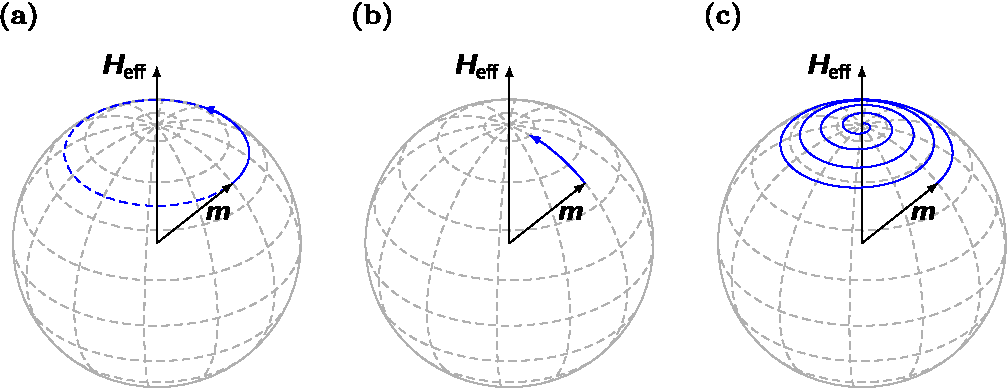
\includegraphics[width=0.9\columnwidth]{Figures/Introduction/abert2013discrete - Figure 2.2.pdf}
    \caption{Motion of a magnetic moment as described by the LLG equation. The motion can be divided into the (a) precessional and (b) damping components. (c) Resulting motion including both precession and damping. Figure taken from~\cite{abert2013discrete}.}
    \label{fig:LLG_motion_Heff}
\end{figure}

\subsubsection{Thermal fluctuations}
% TODO: remove the line in this paragraph that just says where the references come from
The literature in this section comes from the references \cite{LEL-17b}. \par
The LLG equation only takes into account the fundamental physics of the magnetization dynamics at zero temperature. However, in our universe things exist at nonzero temperatures, and thermal fluctuations play an important role in magnetic logic devices. % TODO: when I know what the role is exactly, come back here and tell something small about it here
In order to simulate nanomagnetic structures at nonzero temperatures, Brown~\cite{ThermFluc_SingleDomain} developed a theory to model thermal fluctuations in single-domain particles, by adding a stochastic thermal field $\vb{H_{therm}}$ to the effective field $\vb{H_{eff}}$ in the LLG equation. This thermal field has to fulfill certain statistical properties, namely
\begin{align*}
    \langle \vb{H_{therm}} \rangle &= 0 \mathrm{,} \\
    \langle H_{therm,i}(t) H_{therm,j}(t') \rangle &= q \delta(t-t') \delta_{ij} \mathrm{,}
\end{align*}
where $q=(2 k_B T \alpha)/(M_S \gamma V)$, with $V$ the volume of the single-domain particle. The angled brackets denote either a time average or correlation. With these random and uncorrelated properties of the time-dependent additional field term, the LLG equation becomes a Langevin equation.~\cite{ThermFluc_SingleDomain} However, a nanomagnetic island is not a perfect single-domain particle with uniform magnetization, and different nanomagnetic islands can influence each other through magnetostatic interactions.
Lyberatos~\cite{Lyberatos_1993} realized that every finite-difference cell in a numerical simulation can be seen as one such a single-domain particle, for which Brown's theory can then be applied.~\cite{phd_leliaert} More specifically, the thermal field was implemented in \mumax{}~\cite{LEL-17b,MuMax3} as
\begin{equation}
    \vb{H_{therm}} = \vec{\eta} \sqrt{\frac{2 \alpha k_B T}{M_S \gamma V \Delta t}} \mathrm{,}
    \label{eq:H_therm}
\end{equation}
where $\vec{\eta}$ is a random vector, determined from a standard normal distribution, whose value is changed after every time step. This equation is such that the thermal fluctuations are independent of the spatial discretization (volume $V$ and time step $\Delta t$) used.
% Adaptive time step in mumax problem? Solvers?
There are many finite-difference solvers available in \mumax{}, for example different orders of Runge-Kutta solvers, some of which benefit from the first-same-as-last (FSAL) property. In such solvers, the last torque evaluation of the current step is the same as the first evaluation of the next step, which allows an increase in efficiency because this step only has to be evaluated once. However, the stochastic thermal field is not constant, and hence these solvers can no longer benefit from the FSAL property.~\cite{LEL-17b} Another complication is that the time step $\Delta t$ appears in the expression for $\vb{H_{therm}}$. Since some solvers in \mumax{} improve their efficiency by using an adaptive time step, one must take additional care that the thermal field is calculated correctly in such case. For a detailed description of the implementation of the stochastic thermal field in \mumax{}, we refer to~\cite{LEL-17b}.
% TODO: Can still include something on jump noise process and Curie temperature (phd_leliaert) and a bit more on solvers (start of appendix in phd_leliaert)
% TODO: Find a good place to talk about the advantages of running mumax on gpu, with parallelism etc. (see 'Micromagnetic simulations using Graphics Processing Units')

\section{Tests}
\subsection{Biaxial island}
\label{par:Biaxial_island}
The first part of this thesis consists of investigating the properties of a single biaxial island, as this will be the fundamental building block of more complex circuits. The geometry of such an island is one of the main factors determining the energy barrier between stable states. The geometry under investigation here consists of two ellipses, rotated \SI{90}{\degree} with respect to each other, as shown in \cref{fig:biaxial_island:geometryTypical}. This is chosen because it should be reasonably easy to manufacture as it has no sharp corners. This geometry has two degrees of freedom, namely the long and short axis of the ellipse. We will define the roundness $\rho$ as the ratio between the long and short axis of the ellipses, and the `overall size' $L$ is simply equal to the long axis.
\begin{figure}
    \centering
    
\includegraphics[width=0.3\columnwidth]{Figures/biaxial_island/Geometry/geomPlus55.png}
    \caption{Typical geometry of the biaxial island under investigation, in this specific case for 55x\SI{100}{\nano\metre} ellipses, i.e. $(\rho, L)=(0.55, \SI{100}{\nano\metre})$. White is ferromagnetic material, black is free space.}
    \label{fig:biaxial_island:geometryTypical}
\end{figure}

\subsubsection{Energy barrier}
To determine the energy barrier $E_{barrier}$, the energy landscape as a function of magnetization angle must be calculated. If one were to simply set the magnetization $\vb{M}$ of the entire island in one direction and call it a day, the calculated energy landscape would be flat, due to the absence of the demagnetizing field caused by the shape anisotropy of the magnetic body.~\cite{Nonmonotonic_reversal} Thus, the magnetization should first be relaxed, which can be done using the \mumax{} command \code{minimize()}. However, this would result in a complete relaxation to an energy minimum, hence not yielding any useful information on the energy barrier. To circumvent this issue, an external magnetic field is applied to keep the average magnetization $\frac{1}{A}\int_A \vb{M}\,dA$ close to the initial direction. \par
The procedure is therefore as follows. First the magnetization of the entire island $\vb{M}$ is initialized under one specific angle $\theta$. Then an external magnetic field $B_{ext}$ is applied along that same direction, and the magnetization is relaxed using \code{minimize()}. The internal energy, responsible for the energy landscape, is then equal to $E_{total} - E_{Zeeman}$. This procedure is repeated for different angles $\theta$ to generate an energy profile from which the energy barrier can be deduced. The grid size for these numerical calculations is \SI{1}{\nano\metre} for maximum accuracy.

\paragraph{Optimal simulated external field magnitude}
The procedure as described above makes use of an external magnetic field. It is important to know what the magnitude of this external field should optimally be to determine the energy barrier. To this end, a simulation is carried out in which both the angle $\theta$ and the external magnetic field $B_{ext}$ are varied. In \cref{fig:barrierLandscape-sweepBext} the relaxed magnetization angle is plotted for different magnitudes of the external magnetic field $\abs{\vb{B_{ext}}}$, with the angle of this magnetic field taken at 64 equally spaced values from \SIrange{0}{90}{\degree}.
\begin{figure}
    \centering
    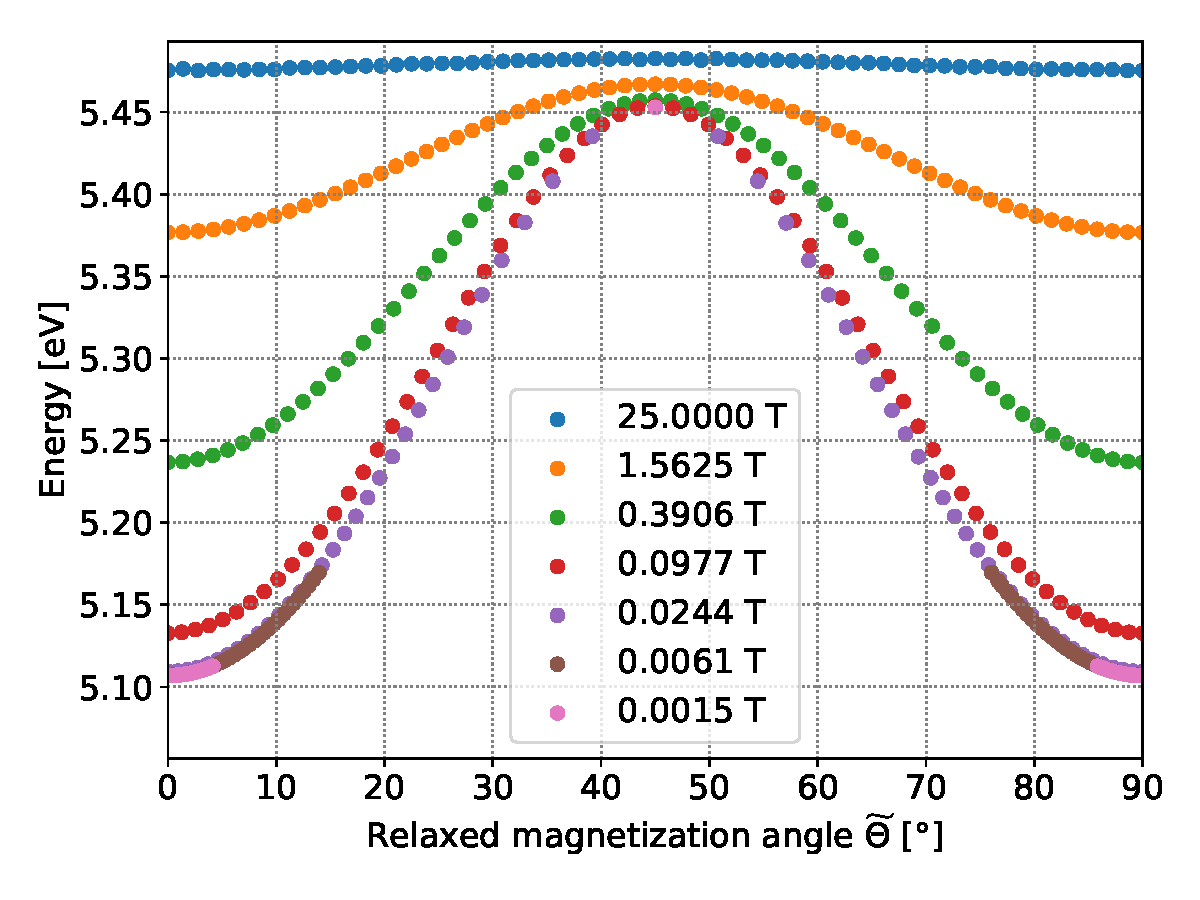
\includegraphics[width=0.9\textwidth]{Figures/biaxial_island/BarrierLandscape/Plus_65_B25-0.001-div4_a128Pi_plotOptimized.pdf}
    \caption{Energy landscape between \SIrange{0}{90}{\degree} for various external magnetic field magnitudes $\abs{\vb{B_{ext}}}$. The external field angle was varied uniformly from \SIrange{0}{90}{\degree} in 64 steps.}
    \label{fig:barrierLandscape-sweepBext}
\end{figure}

Interesting findings:

- Firstly, at very high magnetic fields, the energy landscape is nearly flat as explained earlier.~\cite{Nonmonotonic_reversal}

- Secondly, at an angle of exactly \SI{45}{\degree}, the magnetization remains at the maximum of the energy landscape, which is an unstable equilibrium.

- Thirdly, for lower and lower magnetic field values, the situations for angles very close to \SI{45}{\degree}, the magnetization relaxes to an angle closer to that of the energy minimum. This is to be expected, because lower magnetic fields will have more difficulty keeping the magnetization pointed in the same direction, against the anisotropy.

- Fourthly or finally idk, for lower magnetic fields the energy barrier lowers until it reaches a limit value. This is because high external magnetic fields prevent the relaxation of the edges of the geometry, instead keeping them pointed in roughly the same direction. It is the relaxation of the magnetization angle in a non-uniform way which causes the anisotropy, so forcing the magnetization in a certain direction (like with a high external field) will prevent this from happening, thus increasing the energy and lowering the fictional variant of the energy barrier.

\paragraph{Energy barrier as function of roundness}
See \cref{fig:barrier-cell_size-1nm} blue curve for \SI{128}{\nano\metre}.

\paragraph{Energy barrier as function of overall size}
See \cref{fig:barrier-cell_size-1nm} all different curves

\paragraph{Numerical error: influence of cell size on energy barrier}
When performing longer simulations, it is advantageous to use as large a cell size as possible, to minimize the total amount of cells in the simulation. Increasing the size of the cells does however also increase the numerical error originating from the discretization of the grid. The size of this numerical error was examined by determining the energy barrier for different shapes (varying roundness and overall size) and for different cell sizes of \SI{4}{\nano\metre}, \SI{2}{\nano\metre} and \SI{1}{\nano\metre}. The results of this calculation are shown in \cref{fig:barrier-cell_size}.
\begin{figure}
     \centering
     \begin{subfigure}[b]{0.75\textwidth}
         \centering
         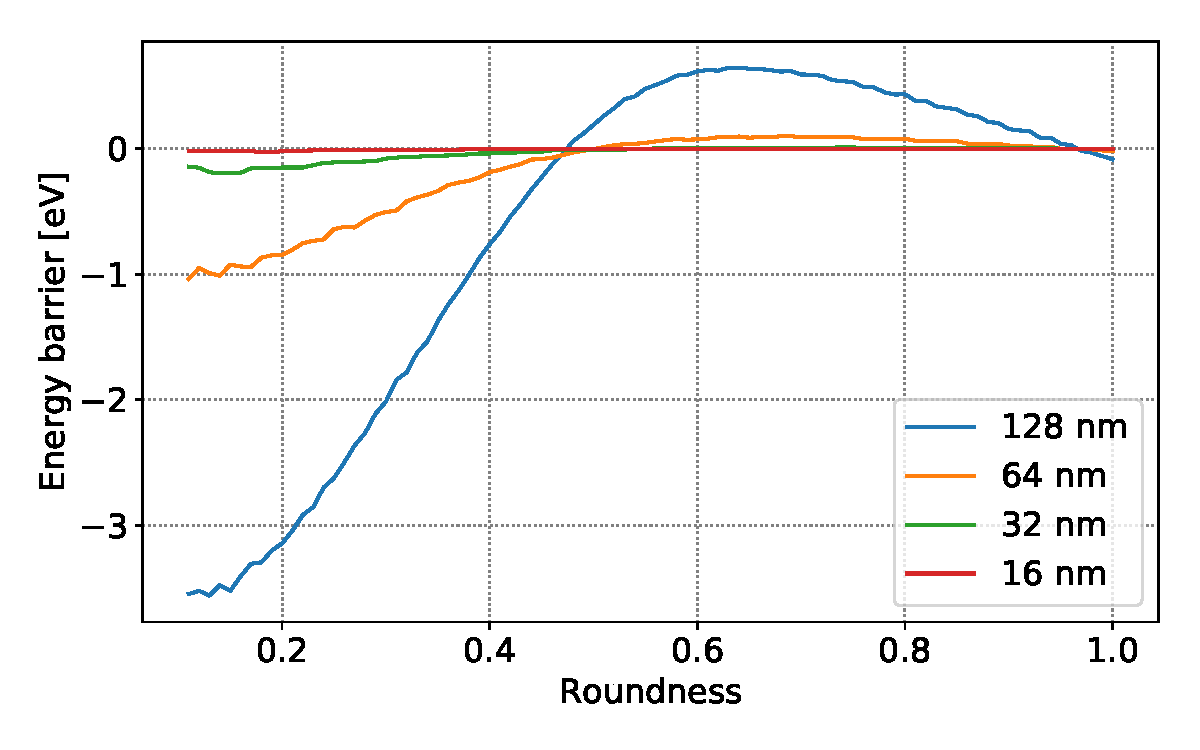
\includegraphics[width=\textwidth]{Figures/biaxial_island/Barrier/Plus_16-128_0.1-1_aPi4_B0.001_cell1nm.pdf}
         \caption{\SI{1}{\nano\metre}}
         \label{fig:barrier-cell_size-1nm}
     \end{subfigure}
     \hfill
     \begin{subfigure}[b]{0.75\textwidth}
         \centering
         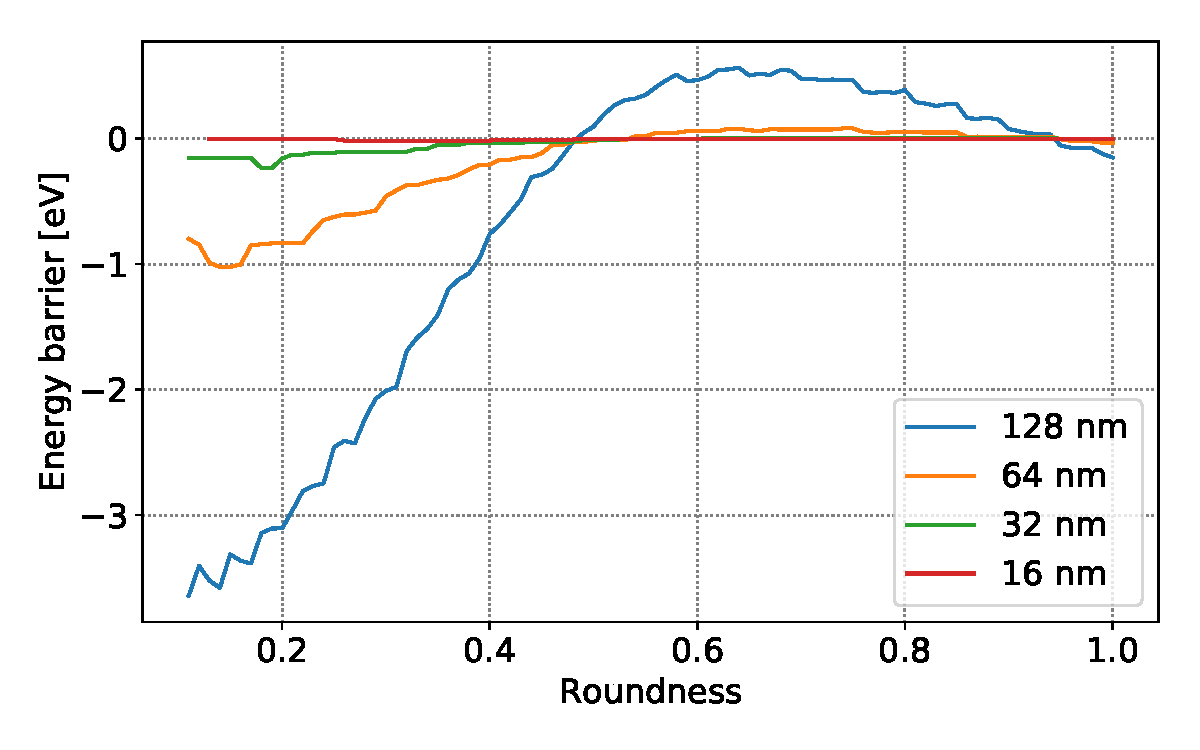
\includegraphics[width=\textwidth]{Figures/biaxial_island/Barrier/Plus_16-128_0.1-1_aPi4_B0.001_cell2nm.pdf}
         \caption{\SI{2}{\nano\metre}}
         \label{fig:barrier-cell_size-2nm}
     \end{subfigure}
     \hfill
     \begin{subfigure}[b]{0.75\textwidth}
         \centering
         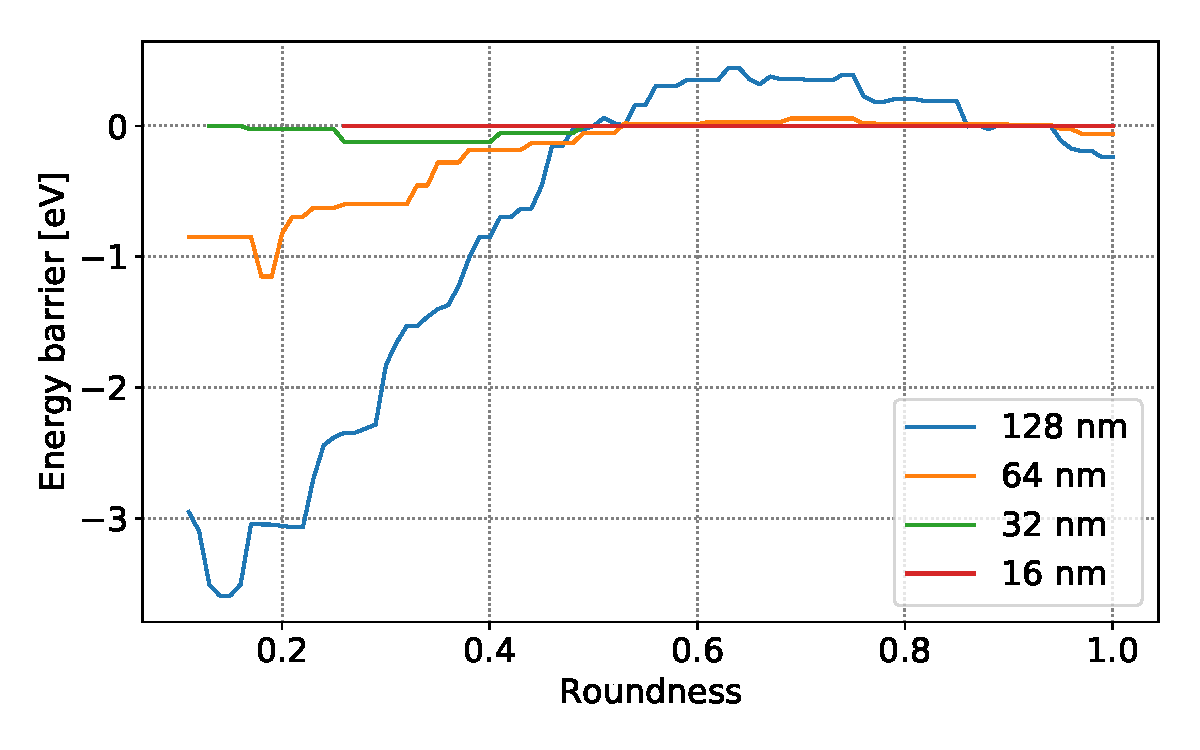
\includegraphics[width=\textwidth]{Figures/biaxial_island/Barrier/Plus_16-128_0.1-1_aPi4_B0.001_cell4nm.pdf}
         \caption{\SI{4}{\nano\metre}}
         \label{fig:barrier-cell_size-4nm}
     \end{subfigure}
        \caption{Energy barrier for different cell sizes. The legend represents the length of the long axis of the ellipses.}
        \label{fig:barrier-cell_size}
\end{figure}
\begin{figure}
    \centering
    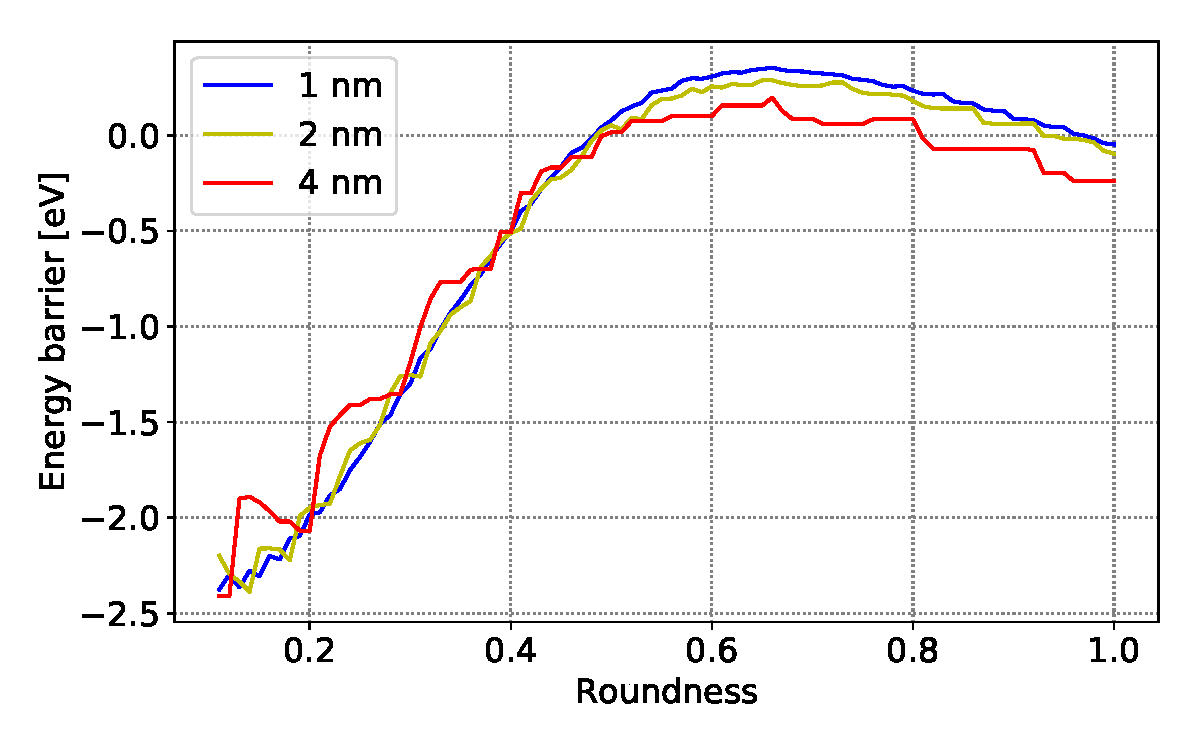
\includegraphics[width=0.9\columnwidth]{Figures/biaxial_island/Barrier/Plus_100_0.1-1_aPi4_B0.001.pdf}
    \caption{Energy barrier for different cell sizes, for a long ellipse axis of \SI{100}{\nano\metre}.}
    \label{fig:barrier-cell_size-100nm}
\end{figure}
The figure obtained with cells of \SI{1}{\nano\metre} is quite smooth, so it is justified that this size was used in the previous paragraphs. For \SI{2}{\nano\metre} cells, the curve becomes rougher, but the overall shape remains very similar to that of \SI{1}{\nano\metre} cells. Cells of \SI{4}{\nano\metre}, however, yield a very rough and almost stair-like energy landscape, which clearly indicates that this size is too large. \par
It may also be noted that for the \SI{4}{\nano\metre} cells, there are no values for the lowest roundnesses for long ellipse axes of \SI{16}{\nano\metre} or \SI{32}{\nano\metre}, because for these situations the short axis is smaller than the grid size, which yields an empty simulation geometry and thus no results. \par
Everything taken into account, it seems that the optimal compromise between simulation speed and accuracy, is a \SI{2}{\nano\metre} cell size, which will be used to perform longer simulations. For the 65x100nm geometry, a \SI{4}{\nano\metre} cell size is probably still acceptable since the energy barrier is similar, and since this will result in a 4x speed increase this will be used. For the perfectly round situation, the difference is very large so it is instructive to use \SI{2}{\nano\metre} or even \SI{1}{\nano\metre}.





% FROM HERE ON THINGS ARE NOT VERY STRUCTURED
\subsection{Random thermal switching}


\subsubsection{Preparation}
\textbf{Step 1: find energy barrier} \\
The procedure used is to set both $m$ and $B_{ext}$ at a certain angle and then \code{minimize()}. Both the magnetic field $B_{ext}$ and the angle $\theta$ are then varied, with $B_{ext}$ going from very high to very low values, and $\theta=0\dots\pi/2$ in steps of $\pi/4$. One could increase the amount of $\theta$-steps, but it is observed that an angle of $\pi/4$ remains magnetized at that angle regardless of the external field, at the very least until $B_{ext} = \SI{0.00153}{\tesla}$. It is however an unstable equilibrium and any slight deviation from this angle will quickly relax to either \SI{0}{\degree} or \SI{90}{\degree} at low fields.
One could even omit the part where theta goes from $\pi/4$ to $\pi/2$ due to symmetry reasons.
All of $\theta = k\frac{\pi}{4} , k\in\mathbb{Z}$ are stable.
At high fields everything is stable and just uniform, which makes the energy landscape flat.

\textbf{Step 2: random switching over \SI{100}{\nano\second}} \\
In GYP-18~\cite{GYP-18} the formula
\begin{equation}
    t_i = -\frac{1}{f_0} \exp(\frac{\Delta E_i}{k_B T}) \ln(1-P_i)
    \label{eq:Switching_time}
\end{equation}
appears, with $f_0 = \SI{e12}{\hertz}$ attempt frequency, and $P_i$ random between 0 and 1. The average value of $-\ln(1-P_i)$ is then $\ln(4) \approx 1.4$.

To get an average $t_i = \SI{100}{\nano\second}$ at $T=\SI{300}{\kelvin}$, one should therefore have
\begin{equation}
    \Delta E_i = k_B T \ln(\frac{f_0 t_i}{\ln(4)}) = 11.19 k_B T = \SI{0.310}{\electronvolt} \mathrm{.}
\end{equation}
The barrier height of a \SI{65}{\nano\metre} elliptic plus-sign geometry is \SI{0.346}{\electronvolt}.
Idea: perhaps attempt frequency is the sinusoidal pattern in the long simulations, with period of about \SI{0.5}{\nano\second}. Observation: This worked with the previous method where $B_{ext}$ was not varied, but with the new (correct) method the $f_0 = \SI{e12}{\hertz}$ works very well again.
Also there is another formula in mumax3~\cite{MuMax3} for uniaxial anisotropy.
% TODO: The gyromagnetic resonance frequency and response time (see ThermFluc_SingleDomain bottom of first page)

\subsubsection{Results}
Step 1: find energy barrier \\
With perfectly circular geometry (i.e. \\
\code{geometry := Ellipse(100e-9, 100e-9)} \\
\code{geometry = geometry.Add(Ellipse(100e-9, 100e-9).RotZ(Pi/2))}) \\
there is still shape anisotropy, but with opposite sign (what are maxima in actual plus-figures are now minima)

Findings (for \SI{100}{\nano\metre} long axis ellipse plus-sign):
at \SI{45}{\nano\metre} the preferred directions switch from the axes (\SI{0}{\degree}) to in between the axes (\SI{45}{\degree}),
at \SI{65}{\nano\metre} the anisotropy with preferred \SI{0}{\degree} direction is the strongest

After running for \SI{1}{\micro\second} at \SI{300}{\kelvin}, with shape \SI{65}{\nano\metre} by \SI{100}{\nano\metre} ellipses in plus shape, the following angles were observed (\cref{fig:switching-alpha}):


\subsubsection{Counting switches}
Since the counting of switches is ambiguous, several different ways of counting them were performed:

1) Counting every crossing of a \SI{90}{\degree} line, e.g. a \SI{270}{\degree} switch is counted as 3 individual switches.

2) Counting every visible switch, with switches larger than \SI{90}{\degree} counted as 1 switch.

3) Looking every \SI{5}{\nano\second} and seeing if the magnetization direction changed without looking at the detailed magnetization in between those timestamps. This excludes 'spikes'.

Formula for $f_0$ derived from \eqref{eq:Switching_time}:
\begin{equation*}
    f_0 = \frac{N \ln(4)}{\Delta t} \exp(\frac{E_{barrier}}{k_B T})
\end{equation*}
with $\Delta t$ the simulation time and $N$ the number of switches.

Formula in \cite{MuMax3} works for the limit of a high barrier compared to the
thermal energy, so perhaps 49x100 is not very representative.

% TODO: This table is too wide, but currently serves as a sort of data storage
The \cref{tab:Switching_f0} is for $\alpha=0.01$:

\ctable[
    cap = Switching Rates,
    caption = {Switching rates and corresponding $f_0$ values for different geometries and grid discretizations, all for $\alpha=0.01$.\\Python: \code{f0 = lambda N, dt, barrier, T: N*math.log(4)/dt*math.exp(barrier/1380649*16021766340/T)}},
    label = {tab:Switching_f0},
    pos = ht,
    sideways
    ]{
    c|c|c|c|c|c|c|c|c|c|c
    }{
    \tnote[a]{The switching rate ($\approx \SI{2}{\nano\second}$) is on the same timescale as the LLG dynamics, hence the exponential relationship of the Arrhenius law is no longer entirely applicable, causing the corresponding values for $f_0$ to be inaccurate. Furthermore, the energy barrier is no longer high compared to the thermal energy, which also reduces the accuracy of the Arrhenius law.}
    }{
        Geom [nm] & Barrier [meV] & Cell [nm] & T [K] & $\Delta t$ [ns] & (1) & (2) & (3) & f0 (1) & f0 (2) & f0 (3) \\
        \hline
        49x100 \tmark[a] & 24.7 & 2 & 300 & 100 & 57 & 37 & 6 & \SI{2.06e9}{} & \SI{1.33e9}{} & \SI{2.16e8}{} \\
        \hline
        65x100 & 155.0 & 4 & 273 & 1000 & 13 & 13 & 9 & \SI{1.31e10}{} & \SI{1.31e10}{} & \SI{9.06e9}{} \\
        65x100 & 155.0 & 4 & 300 & 1000 & 15 & 11 & 7 & \SI{8.35e9}{} & \SI{6.12e9}{} & \SI{3.89e9}{} \\
        65x100 & 155.0 & 4 & 350 & 1000 & 51 & 41 & 30 & \SI{1.21e10}{} & \SI{9.69e9}{} & \SI{7.09e9}{} \\
        65x100 & 286.0 & 2 & 350 & 500 & 0 & 0 & 0 & 0 & 0 & 0 \\
        65x100 & 207.9 & 3.125 & 350 & 1000 & 12 & 9 & 7 & \SI{1.64e10}{} & \SI{1.23e10}{} & \SI{9.56e9}{} \\
        \hline
        100x100 & 241.1 & 4 & 300 & 1000 & 0 & 0 & 0 & 0 & 0 & 0 \\
        100x100 & 241.1 & 4 & 350 & 1000 & 5 & 5 & 5 & \SI{2.06e10}{} & \SI{2.06e10}{} & \SI{2.06e10}{} 
    }


\begin{figure}
     \centering
     \begin{subfigure}[b]{0.75\textwidth}
         \centering
         \includegraphics[width=\textwidth]{Figures/biaxial_island/Switching/65x100_300K_alpha0.1_1µs_4nm.pdf}
         \caption{$\alpha=0.1$}
         \label{fig:switching-alpha-0.1}
     \end{subfigure}
     \hfill
     \begin{subfigure}[b]{0.75\textwidth}
         \centering
         \includegraphics[width=\textwidth]{Figures/biaxial_island/Switching/65x100_300K_alpha0.01_1µs_4nm.pdf}
         \caption{$\alpha = 0.01$}
         \label{fig:switching-alpha-0.01}
     \end{subfigure}
        \caption{Switching for different $\alpha$, with grid discritization of \SI{4}{\nano\metre} at \SI{300}{\kelvin}, for 65x100.}
        \label{fig:switching-alpha}
\end{figure}

\begin{figure}
     \centering
     \begin{subfigure}[b]{0.49\textwidth}
         \centering
         \includegraphics[width=\textwidth]{Figures/biaxial_island/Switching/65x100_300K_alpha0.01_1µs_4nm.pdf}
         \caption{\SI{300}{\kelvin}, 65x100}
         \label{fig:switching-temp-300-65x100}
     \end{subfigure}
     \hfill
     \begin{subfigure}[b]{0.49\textwidth}
         \centering
         \includegraphics[width=\textwidth]{Figures/biaxial_island/Switching/65x100_350K_alpha0.01_1µs_4nm.pdf}
         \caption{\SI{350}{\kelvin}, 65x100}
         \label{fig:switching-temp-350-65x100}
     \end{subfigure}
     \begin{subfigure}[b]{0.49\textwidth}
         \centering
         \includegraphics[width=\textwidth]{Figures/biaxial_island/Switching/100x100_300K_alpha0.01_1µs_4nm.pdf}
         \caption{\SI{300}{\kelvin}, 100x100}
         \label{fig:switching-temp-300-100x100}
     \end{subfigure}
     \hfill
     \begin{subfigure}[b]{0.49\textwidth}
         \centering
         \includegraphics[width=\textwidth]{Figures/biaxial_island/Switching/100x100_350K_alpha0.01_1µs_4nm.pdf}
         \caption{\SI{350}{\kelvin}, 100x100}
         \label{fig:switching-temp-350-100x100}
     \end{subfigure}
    \caption{Switching for different temperatures, with grid discritization of \SI{4}{\nano\metre} and $\alpha = 0.01$.}
    \label{fig:switching-temp}
\end{figure}
\begin{figure}
    \centering
    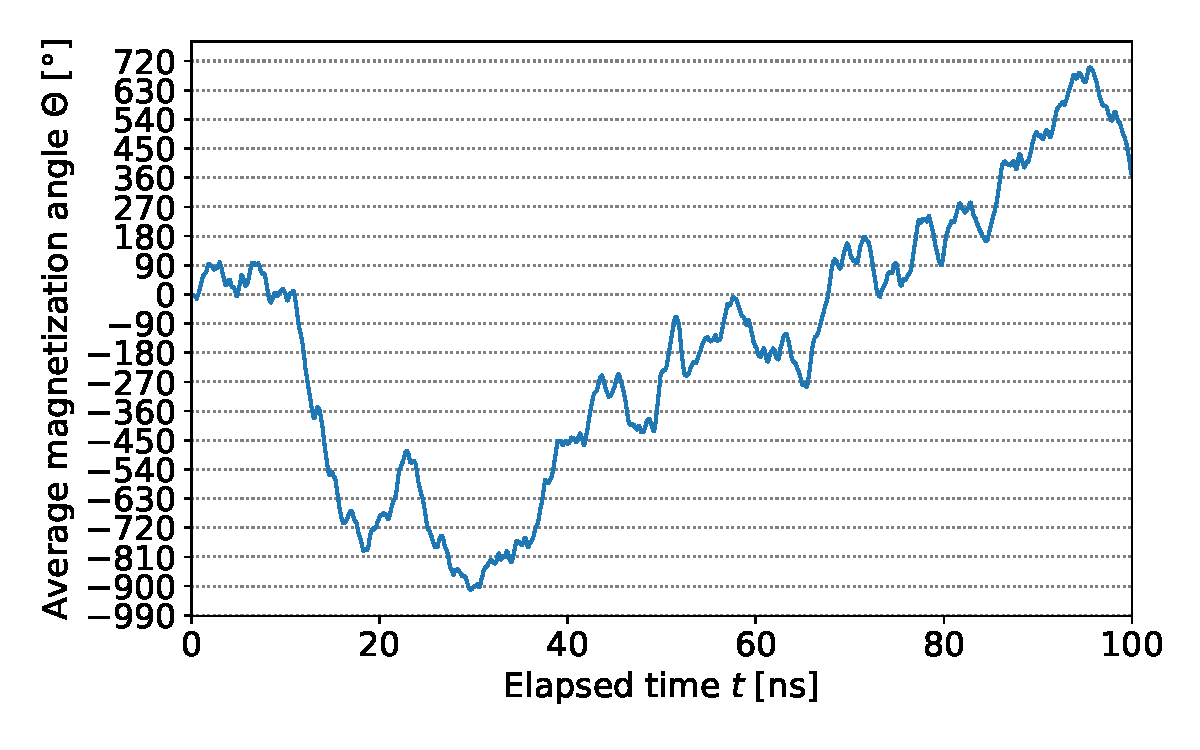
\includegraphics[width=0.9\columnwidth]{Figures/biaxial_island/Switching/49x100_300K_alpha0.01_100ns_2nm.pdf}
    \caption{Switching for a long ellipse axis of \SI{49}{\nano\metre}, which has a very low energy barrier, with grid discretization of \SI{2}{\nano\metre} at \SI{300}{\kelvin} and $\alpha = 0.01$.}
    \label{fig:switching-49x100-300}
\end{figure}

\subsection{External field}
\begin{figure}
     \centering
     \begin{subfigure}[b]{0.65\textwidth}
         \centering
         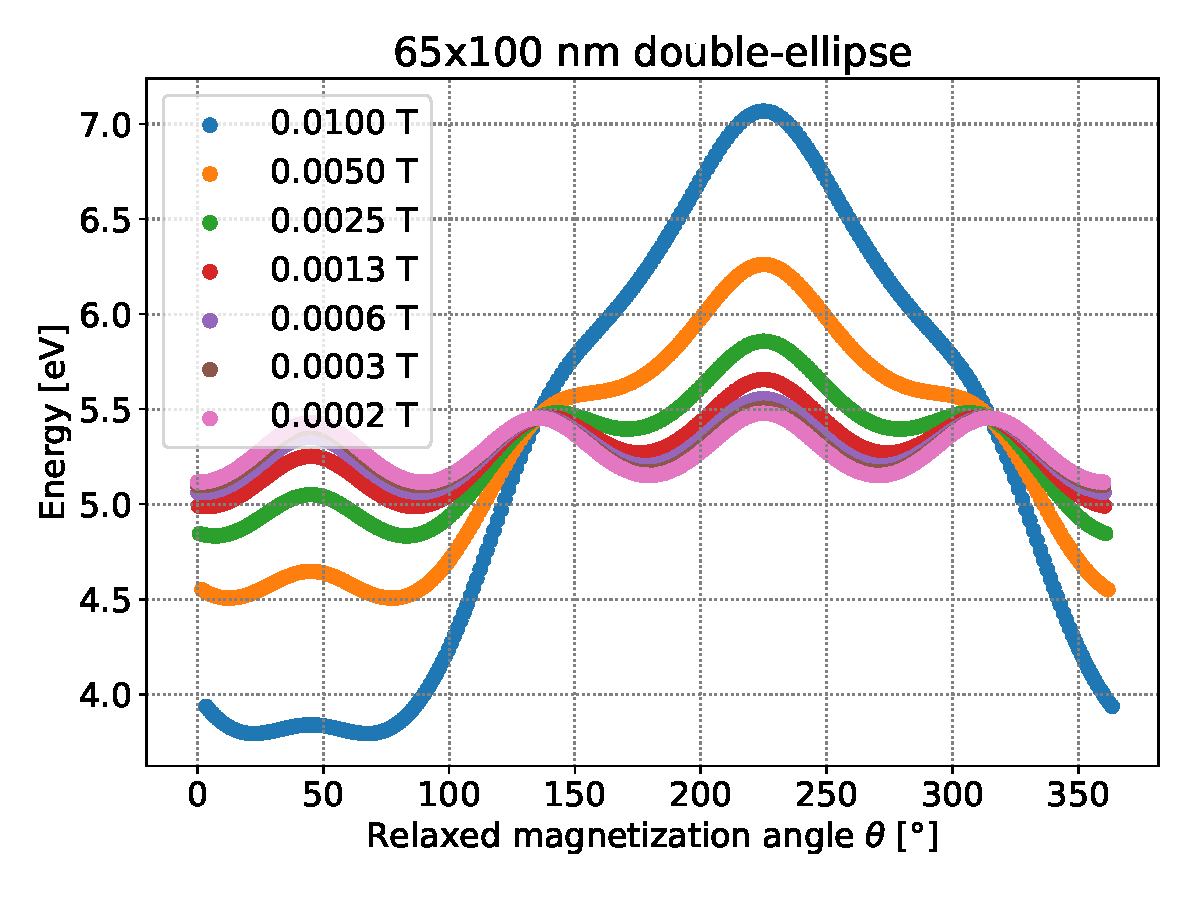
\includegraphics[width=\textwidth]{Figures/biaxial_island/BarrierLandscape/Ext_K0.1Ms2_Bext1e-2-1e-4_aPi4.pdf}
         \caption{External angle $\pi/4$}
         \label{fig:barrierLandscape-externalAngle-pi4}
     \end{subfigure}
     \hfill
     \begin{subfigure}[b]{0.65\textwidth}
         \centering
         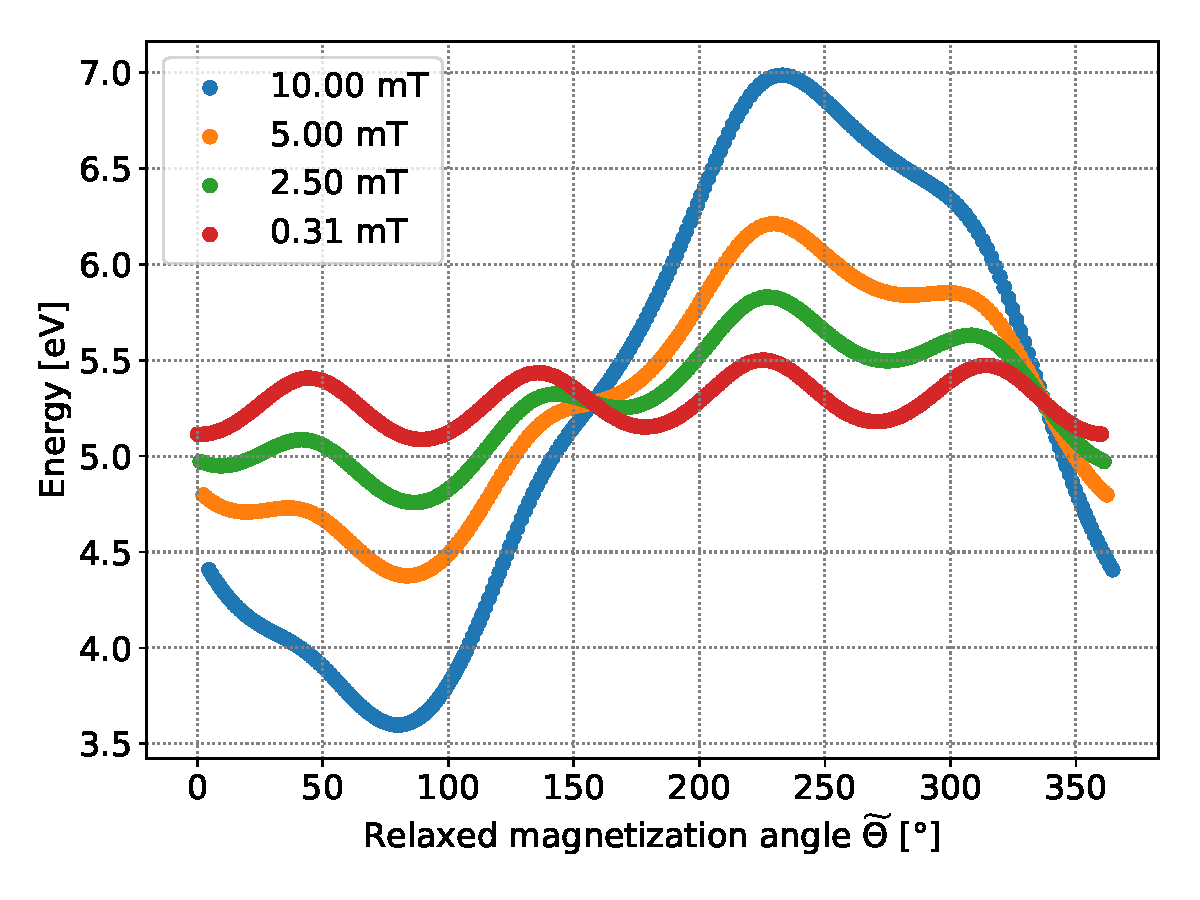
\includegraphics[width=\textwidth]{Figures/biaxial_island/BarrierLandscape/Ext_K0.1Ms2_Bext1e-2-1e-4_a3Pi8.pdf}
         \caption{External angle $3\pi/8$}
         \label{fig:barrierLandscape-externalAngle-3pi8}
     \end{subfigure}
     \begin{subfigure}[b]{0.65\textwidth}
         \centering
         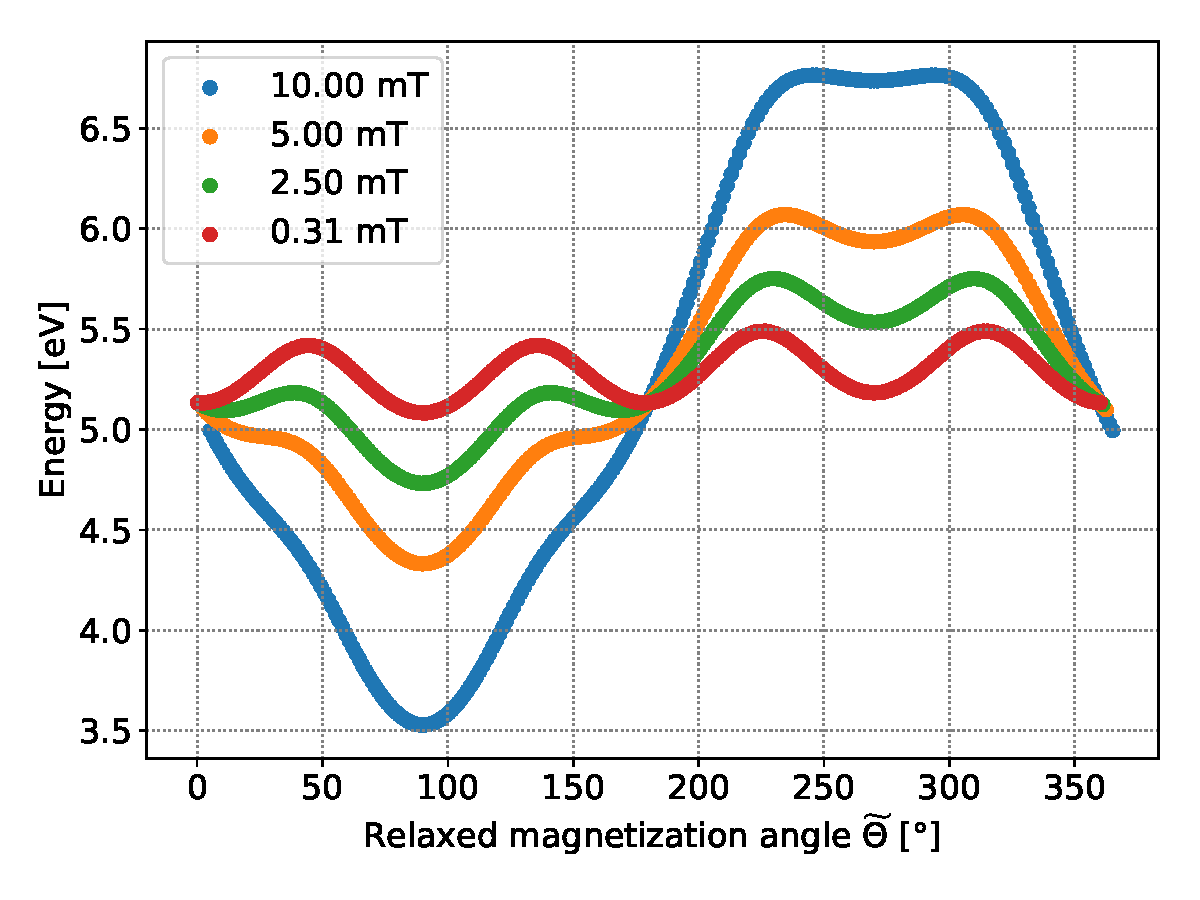
\includegraphics[width=\textwidth]{Figures/biaxial_island/BarrierLandscape/Ext_K0.1Ms2_Bext1e-2-1e-4_aPi2.pdf}
         \caption{External angle $\pi/2$}
         \label{fig:barrierLandscape-externalAngle-pi2}
     \end{subfigure}
     \hfill
    \caption{Energy landscape for different external field angles (plots a, b, c), and different external field strengths (legend).}
    \label{fig:barrierLandscape-externalAngle}
\end{figure}


\newpage
\bibliographystyle{IEEEtran}
\bibliography{bibliography/bibliography.bib}


\end{document}
